\documentclass[../main.tex]{subfiles}
\begin{document}
Linux è un sistema operativo \textbf{multiutente}. Per autenticarsi c'è bisogno di un nome utente (che è univoco) e una password.
La lista di tutti gli utenti è disponobile nel file \code{/etc/passwd}. L'utente \code{root} ha tutti i privilegi di sistema.

Gli utenti possono essere organizzati in gruppi, la lista di tutti i gruppi è disponobile nel file \code{/etc/groups}, di base
ogni utente viene anche inserito in un gruppo con il suo nome. Ovviamente un utente può appartenere a più gruppi ma si è attivi
in un unico gruppo alla volta.

\begin{figure}[h]
    \centering
    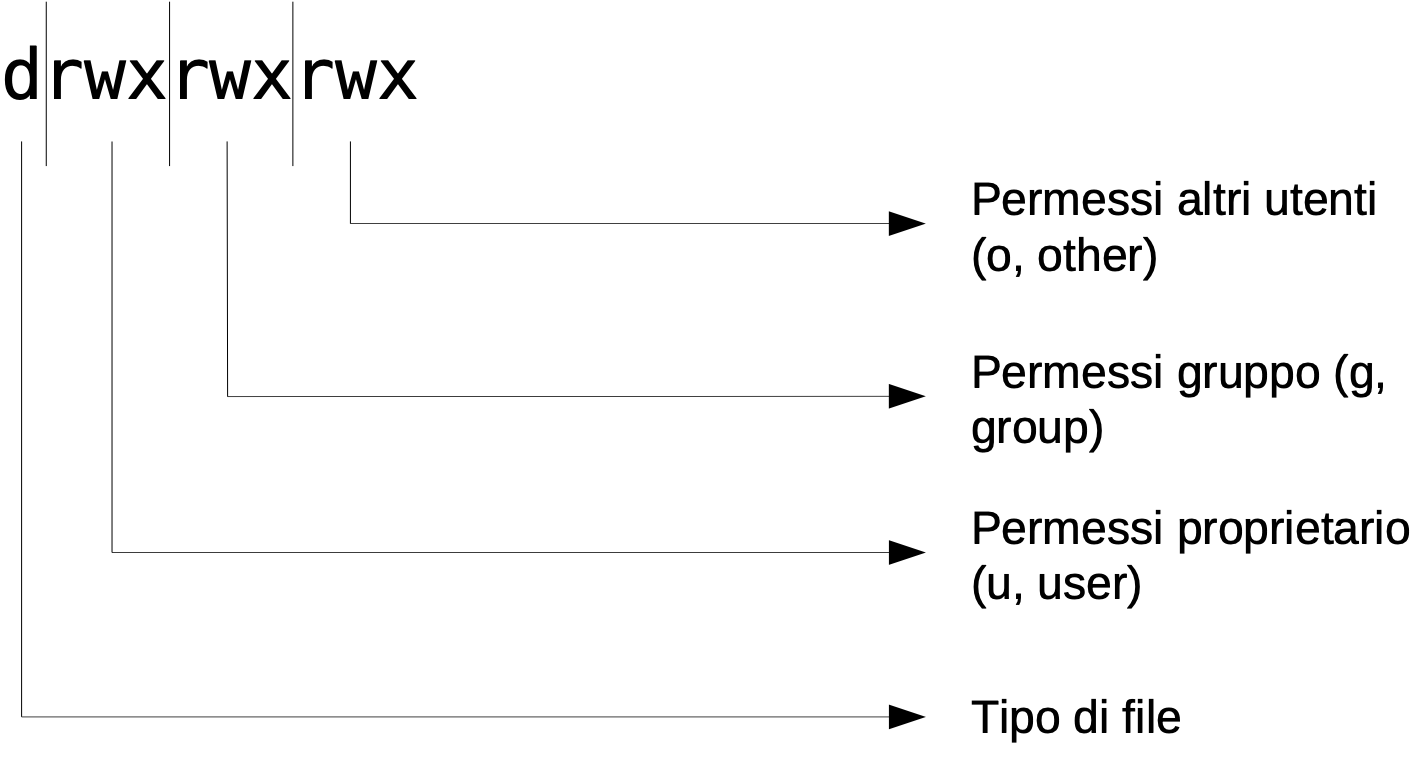
\includegraphics[width=0.6\textwidth]{../images/permessi.png}
    \caption{Struttura dei permessi}
\end{figure}
\textbf{Nota:} ci sono diversi tipi di file ma generalmente ci sarà \code{d} (directory) o \code{-} (file regolare).

\vspace{0.5cm}
Se l'immagine di prima rappresentava la struttura dei permessi, ora cerchiamo di descrivere i permessi di base e come si comportano
su file e directory:
\begin{itemize}
    \item \textbf{Lettura (r)}
    \begin{itemize}
        \item \textit{File: } permette di leggerne il conenuto
        \item \textit{Directory: } permette di elencarne il contenuto (file, sotto-directory)
    \end{itemize}
    \item \textbf{Scrittura (w)}
    \begin{itemize}
        \item \textit{File: } permette di modificarne il conenuto
        \item \textit{Directory: } permette di aggiungere o rimuovere contenuto
        \begin{itemize}
            \item posso cancellare un file solo se ho permessi sulla directory che lo contiene, \underline{non basta} il permesso di scrittura sul file
        \end{itemize}
    \end{itemize}
    \item \textbf{esecuzione (x)}
    \begin{itemize}
        \item \textit{File: } permette di eseguirli (su un file .txt ad esempio è inutile)
        \item \textit{Directory: } permette di attraversarle per accedere a file e sotto-directory, non permette di elencare il contenuto
    \end{itemize}
\end{itemize}

\subsubsection{Cambiare i permessi}
Ci sono due modi per cambiare i permessi:
\begin{itemize}
    \item Modalità simbolica, \code{chmod [-R] [ugo] [+-=] [rwxst] files}
    \item Modalità ottale, \code{chmod [-R] [N][N][N][N] files}
\end{itemize}
\textbf{Nota:} \code{ugo} indica (user, group, others)

\textbf{Nota:} nella modalità ottale i permessi vengono rappresentati con dei bit, in generale \code{r} vale 4, \code{w} 2 e \code{x} 1

È inoltre possibile cambiare il proprietario di un file con \code{chown} e cambiare il gruppo di un file con \code{chgrp}
\end{document}